\chapter{Results and Interpretation}

\section{Parameters and Nondimensionalization}

For most analyses, many of the parameters and results are non-dimensionalized. In
particular, instead of separate parameters for \(k_z\) and \(k_{xy}\), \(k_z\)
and \(k_{\textrm{meas}}\) are both normalized by \(k_{xy}\). Numerical
experiments verified that this is permissible, as numerical experiments with
different \(k_z\) and \(k_{xy}\) parameters but equivalent ratios
\(\fracflat{k_z}{k_{xy}}\) resulted in very similar ratios of
\(\fracflat{k_{\textrm{meas}}}{k_{xy}}\).

Angle is an exception. In this analysis, all angles are given as degrees from
the horizontal (\(xy\)) plane.

\section{Numerical vs. Analytical Predictions}

A 3-D plot of the numerical and analytical predictions may be seen in 
Figure \ref{fig:numvanal}.

\begin{figure}[h]
\centering
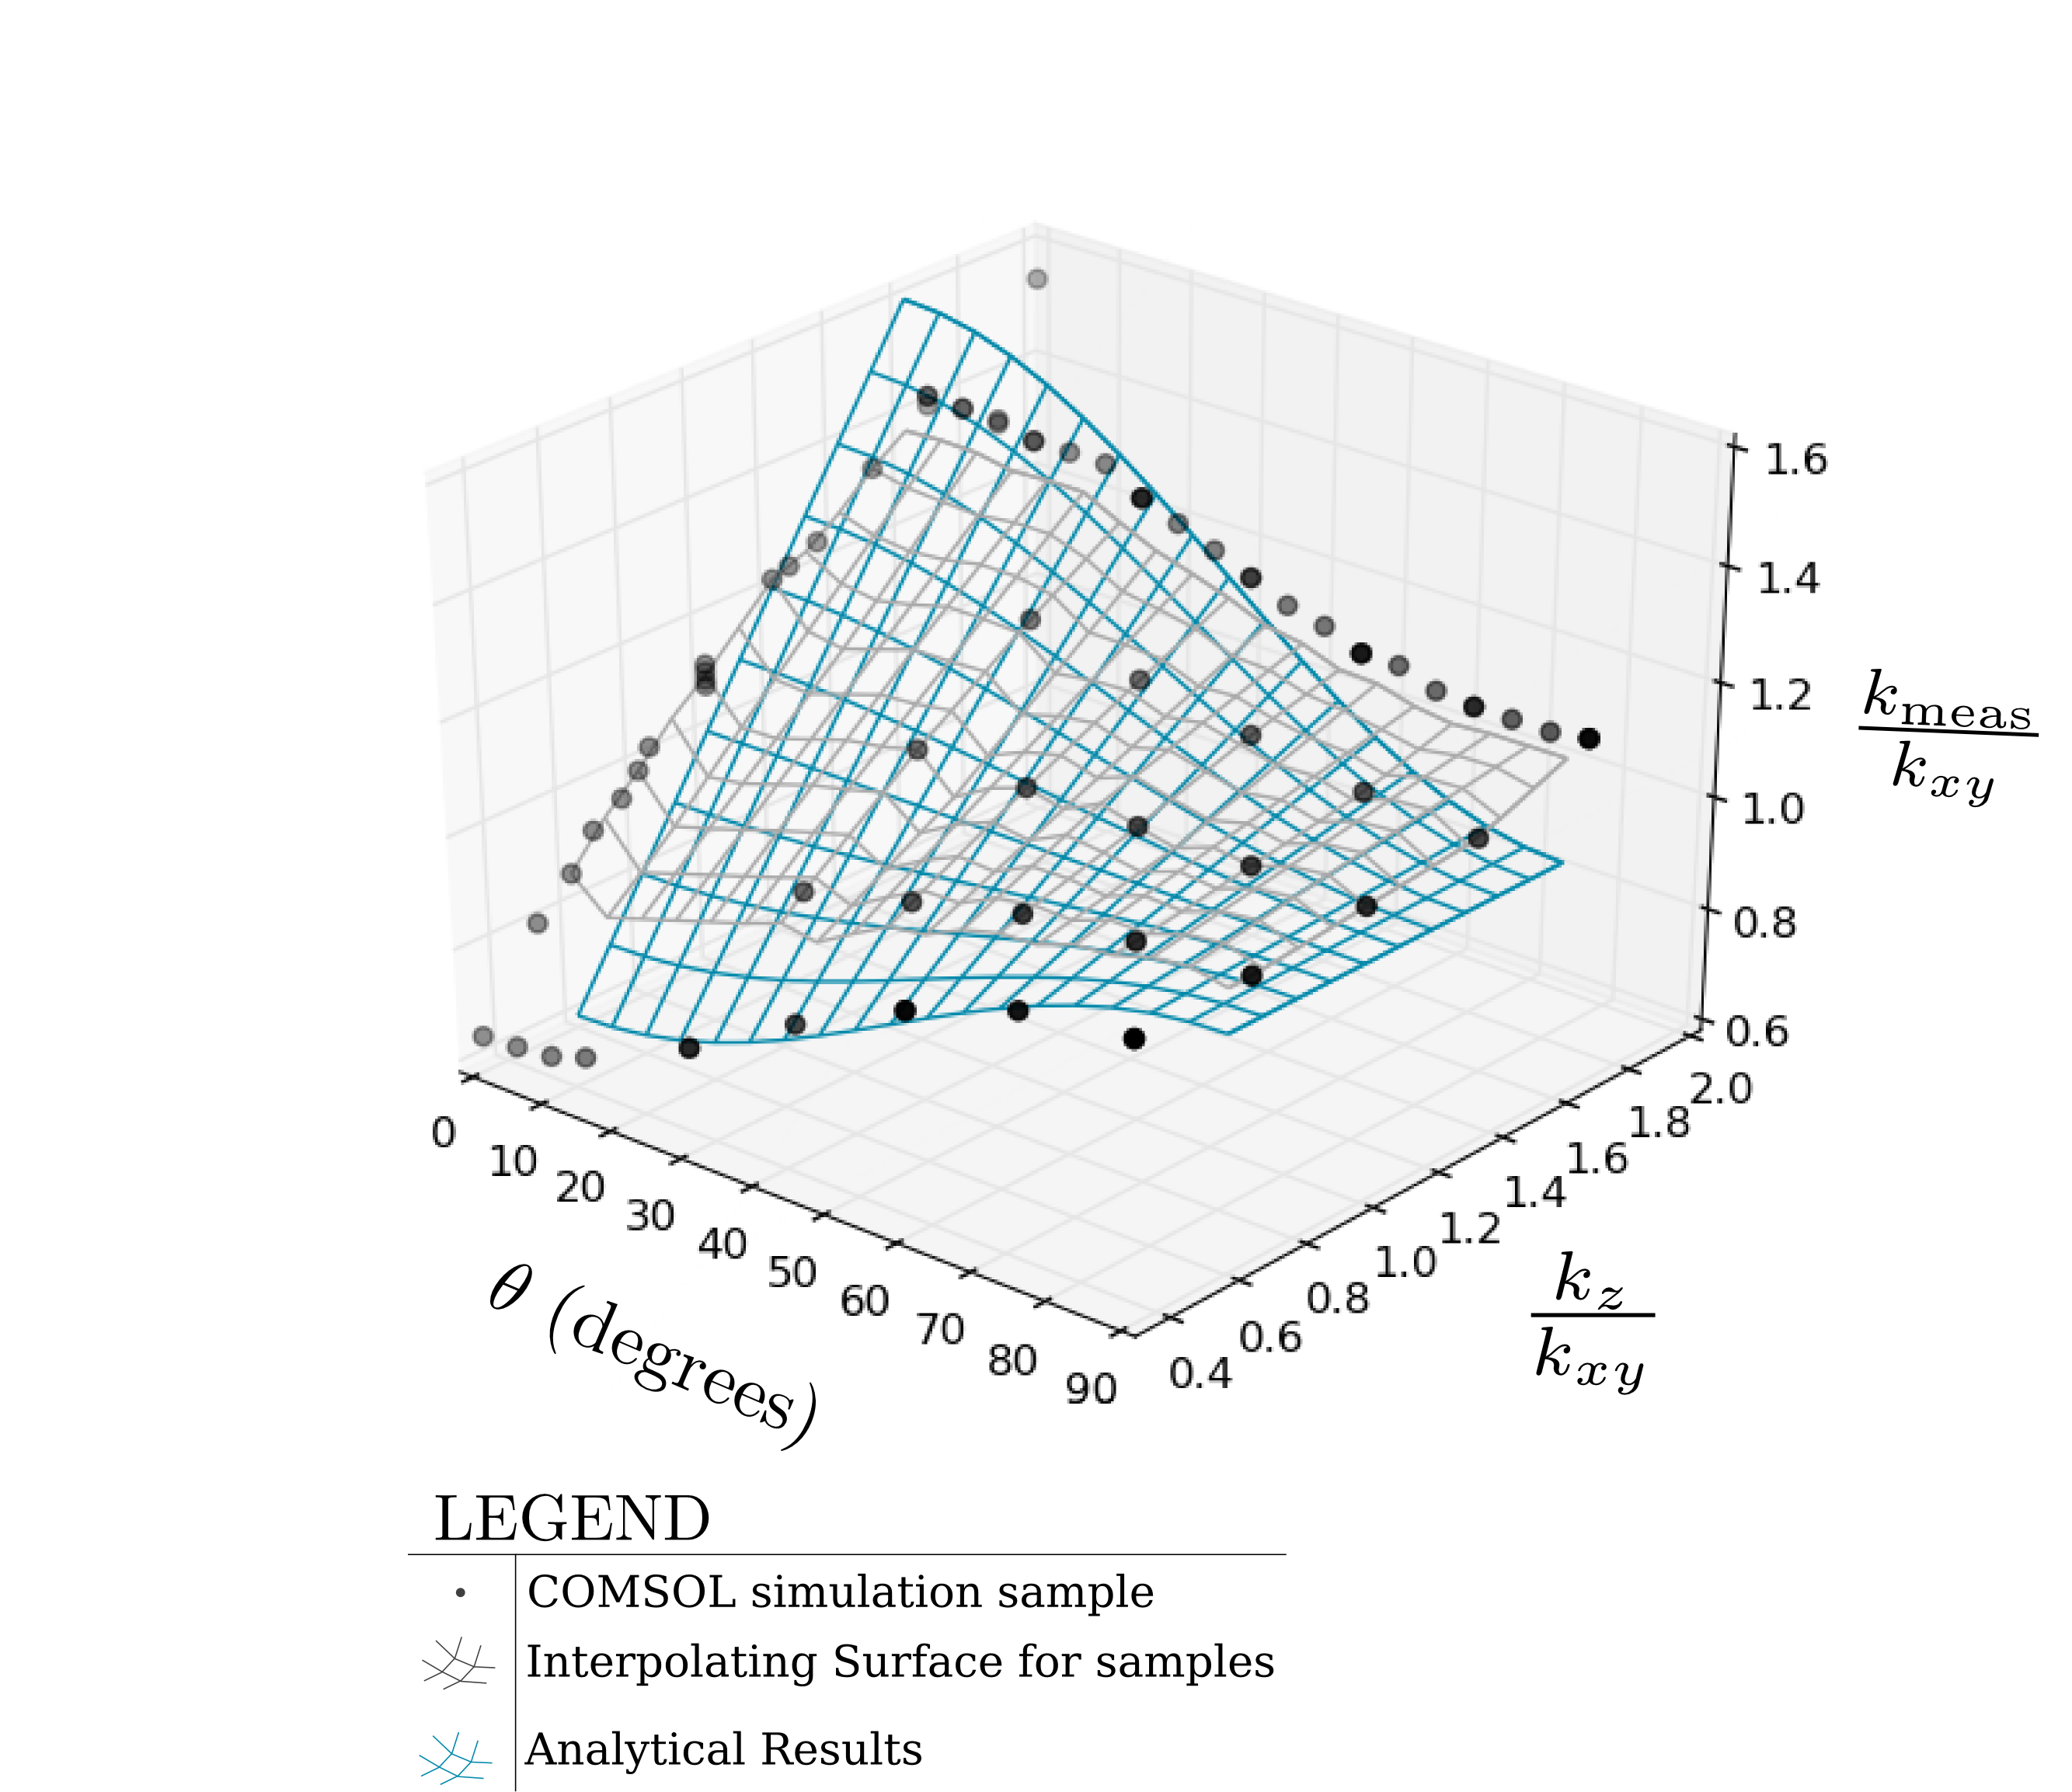
\includegraphics[width=\textwidth]{fig/numvanal.png}
\caption{A comparison of the numerical results and the analytical theory shows
general agreement. Grey dots represent numerical simulation results, the grey surface represents an interpolating surface of the dots, and the blue surface represents the analytical model. Disagreement between the two may be due to edge effects and/or numerical
model convergence issues.}
\label{fig:numvanal}
\end{figure}

This plot shows that the two approaches to predicting measured conductivity
as a function of angle and anisotropy ratio are in general agreement. However,
there are subtle disagreements which may be important. For example, the
numerical model predicts overreporting of the thermal conductivity for
isotropic materials by about \(10\%\), and generally predicts smoother
curves for strongly anisotropic materials than the analytical approach.

There are two potential explanations for this: The first has to do with edge
effects, while the second has to do with convergence properties of the numerical
model.

In the first case, the numerical model accounts for edge effects by
modeling a finite length needle. Meanwhile, the analytical model does not take
into account edge effects, as it models an infinitely long needle like the
original needle probe method. The author conjectures that this is the mechanism
primarily responsible for the smoothing of \(k_{\textrm{meas}}(\theta)\) at more extreme
cases of anisotropy. In fact, for the isotropic case, these edge effects have
been studied and quantified analytically by other researchers. \cite{axialerror}


In the second case, the numerical model operates with a moderately coarse grid.
The convergence study results show that, while the time/temperature curves look
largely the same (Figure \ref{fig:conv_curves}), that the minor differences are magnified when taking the
derivative with respect to \(\ln(t)\) such that the coarse grid reports a
thermal conductivity of about \(110\%\) of the finer grid (Table \ref{tab:conv_kvals}). The author
conjectures that such effects may explain why the numerical predictions
consistently over-predict thermal conductivity as compared to the analytical
predictions, particularly in the isotropic case.


\begin{figure}[h]
\centering
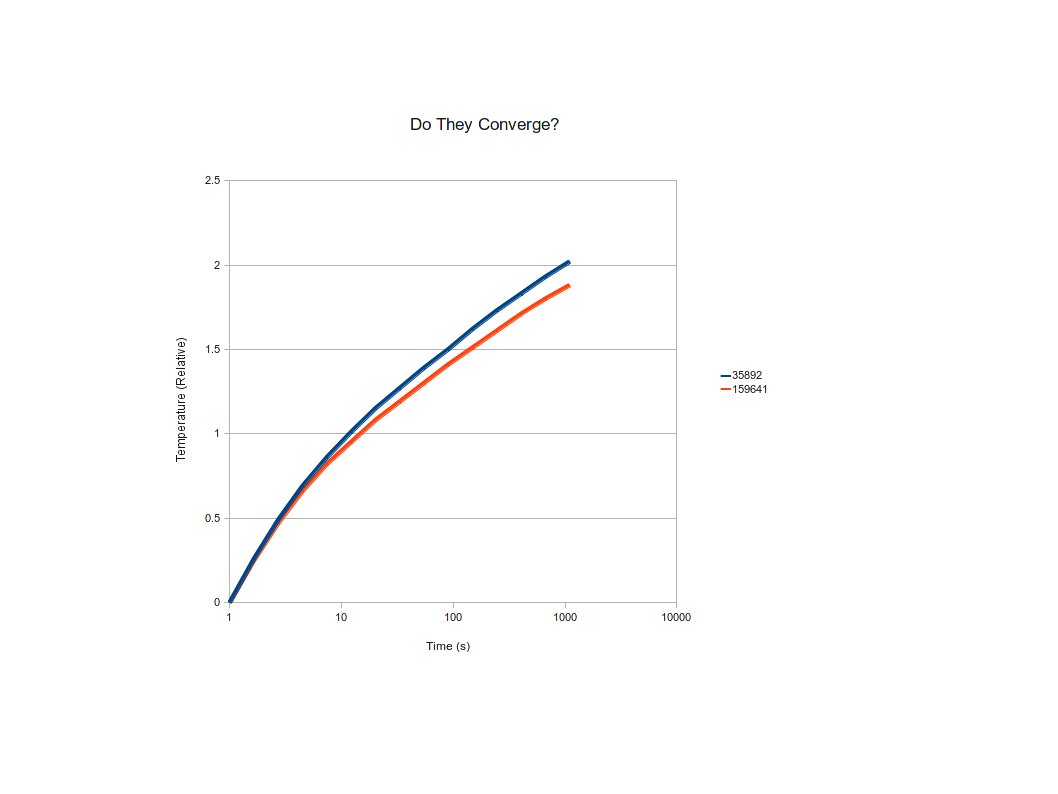
\includegraphics[width=0.6\textwidth]{fig/conv_curves.png}
\caption{A comparison of two \(T(t)\) curves from equivalent simulations with 
different fineness of mesh. These two curves appear quite similar, but their long-
time slopes are measurably different}
\label{fig:conv_curves}
\end{figure}


\begin{table}[h]
\centering
\begin{tabular}{r | l}
 & Slope\\
\(35892\) elements & 0.215\\
\(159641\) elements & 0.198\\
\% Error & 8.64 \%
\end{tabular}

\caption{A comparison of \(k_{\textrm{meas}}\) from two equivalent simulations 
with different fineness of mesh. Despite the similarities in time/temperature
curves, the resulting  conductivity calculations differ by nearly 10 \%. Units are in W\(/\)m\(\cdot\)K.}
\label{tab:conv_kvals}
\end{table}

\section{Benchtop Measurements}

The results of the benchtop measurements are mixed.

\begin{figure}[h]
\centering
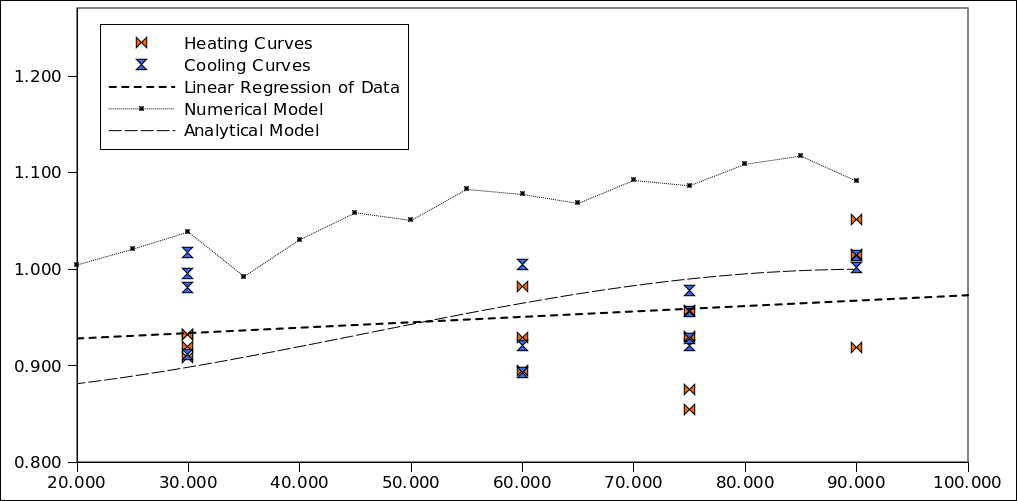
\includegraphics[width=0.9\textwidth]{fig/test_results.png}
\caption{A comparison of the benchtop measurements with the numerical and
analytical predictions, given the calculated anisotropic thermal conductivity.}
\label{fig:test_results}
\end{figure}

\begin{table}[h]
\centering
\begin{tabular}{l l | l l}
Angle (degrees) & # & Heating & Cooling\\
90 & 1 & 0.223284242942 & 0.243481576262\\
& 2 & 0.246684312618 & 0.24641641198\\
& 3 & 0.255505537961 & \sout{0.318256880271}\\
75 & 1 & 0.212791418373 & 0.223684883264\\
& 2 & 0.2325853424 & 0.232407779425\\
& 3 & 0.207604305022 & 0.225508200642\\
& 4 & 0.22608462065 & 0.237662896347\\
60 & 2 & 0.238543591267 & 0.244064408529\\
& 3 & 0.225850168518 & 0.22374914604\\
& 4 & 0.217518339596 & 0.216990054548\\
30 & 1 & 0.226573190917 & 0.238313150421\\
& 2 & 0.226429675463 & 0.247135960358\\
& 3 & 0.220619372302 & 0.241951060919\\
& 4 & 0.223387867071 & 0.221486604074\\
\end{tabular}

\caption{Raw data from the benchtop measurements. Note that one of the cooling curve measurements is striked out. This is because, when examined, it is clearly an outlier. Units are in W\(/\)m\(\cdot\)K.}
\label{tab:powders}
\end{table}


\begin{figure}[h]
\centering
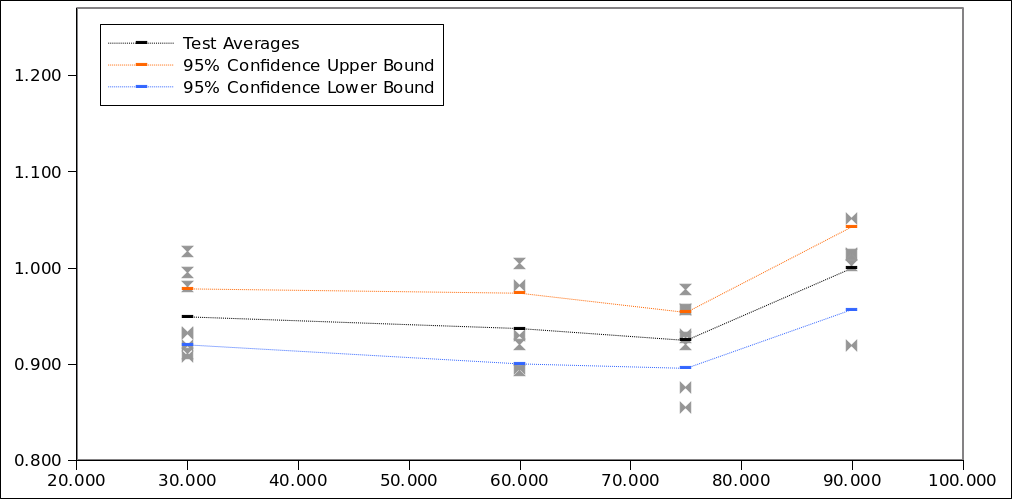
\includegraphics[width=0.9\textwidth]{fig/test_results_confidence.png}
\caption{Upper and lower bounds of 95 \% confidence in measurements. This analysis 
indicates that the measurements can not statistically exclude a null hypothesis.}
\label{fig:test_confidence}
\end{figure}

\begin{table}[h]
\centering
\begin{tabular}{r | l l l}
 & \multicolumn{3}{c}{ \(k_{\textrm{meas}} / \bar{k_{xy}}\) }\\
Angle & Mean & Standard Deviation & 95\% Confidence\\
90 & 1.000 & 0.0491 & 0.0431\\
75 & 0.923 & 0.0419 & 0.0291\\
60 & 0.937 & 0.0459 & 0.0367\\
30 & 0.949 & 0.0420 & 0.0291\\
\end{tabular}

\caption{Basic statistics on normalized benchtop measurements.  Units are in W\(/\)m\(\cdot\)K.}
\label{tab:pow-stats}
\end{table}


First, it may be seen that there is a significant amount of noise inherent in
the needle probe method, even accounting for obviously failed measurements.
This is likely due in part to the numerical derivative as well as the relatively
unpredictable behavior of porous materials. Given
this noise, it is difficult to see which of the two models is more appropriate.

Based on a general curve fit, the results show a slight upward slope, as
expected. However, given the variation in the results, it is statistically
possible that angle has absolutely no effect on the reading. This could be fixed
with more careful, exacting standards in the construction of the anisotropic
materials, more measurements at each angle, and measurements at more angles.
In other words, given the variance of the measurements, many more measurements
would have to be made in order to reach any statistically significant
conclusions, at least given the relatively amount of anisotropy of the sample.

Also given this noise and the relatively weak levels of anisotropy in the
sample, even with more measurements, it could still prove difficult to deduce
the degree of anisotropy of the sample with this data and a curve fit to either
the numerical or analytical predictions alone.

\section{In-Situ Snow Measurements}

% This would be a good thing for an appendix.
\begin{comment}
\begin{table}[h]
\centering
\begin{tabular}{l | l l}
\# & h (inches) & Angle (degrees)
5 & 10.5 & 85\\
6 & 10.5 & 85\\
7 & 13 & 38\\
8 & 12.5 & 45\\
9 & 10.5 & 92
\end{tabular}

\label{tab:metadata}
\caption{Height and angle measurements from snow measurements. The height data was unused in this analysis.}
\end{table}
\end{comment}

\begin{table}[h]
\centering
\begin{tabular}{r | l l}
Angle & Heating & Cooling\\
0 & 0.0289 & 0.0321\\
5 & 0.0269 & 0.0244\\
45 & 0.0290 & 0.0327\\
52 & 0.0288 & 0.0326\\
\end{tabular}

\caption{Conductivity results from the snow measurements. Units are in W\(/\)m\(\cdot\)K.}
\label{tab:snow}
\end{table}

\begin{table}[h]
\centering
\begin{tabular}{r | l}
Control Volume & \(736.76\) mL\\
Mass & \(161.14\) g\\
Density & \(0.219\) g/mL\\
& 219 kg/\(\textrm{m}^3\)\\
\end{tabular}

\caption{Measured and derived measurements for snow density. Units are in W\(/\)m\(\cdot\)K.}
\label{tab:density}
\end{table}

\begin{figure}[h]
\centering
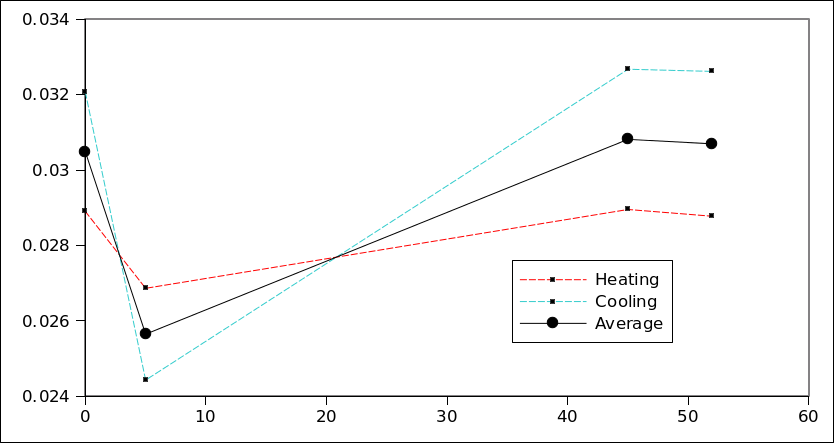
\includegraphics[width=0.9\textwidth]{fig/snow_meas.png}
\caption{Conductivity measurements in roughly the same layer of snow at various 
angles. Even a limited amount of in-situ snow measurements suggest a degree of
anisotropy.}
\label{fig:snow_results}
\end{figure}

\begin{figure}[h]
\centering
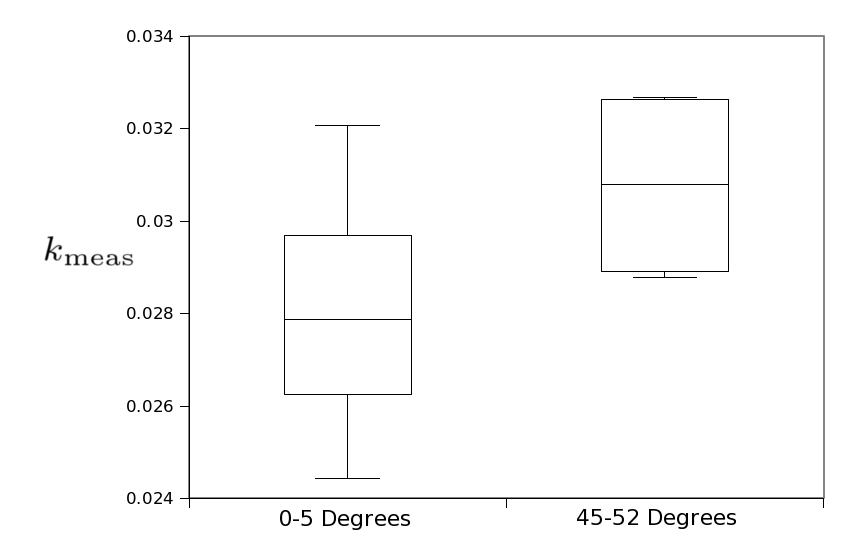
\includegraphics[width=0.9\textwidth]{fig/snow_meas_boxplot.png}
\caption{These boxplots give a general idea of the differences in measurements
between the near-horizontal angle and the more oblique ones in snow.}
\label{fig:test_boxplot}
\end{figure}


Due to the difficulty in taking snow measurements on top of the inherent noise
of the method, snow measurements are also inconclusive. However, the
measurements taken \emph{do} indicate anisotropy to a greater degree of confidence
than the benchtop measurements. Like the case of the benchtop measurements, with so few
measurements a curve fit against either method of prediction is unlikely to
yield useful results.
